% !TeX root = ../main.tex
% Bảy biểu đồ từ output notebook bước 1--6 và một ảnh chụp dashboard thực tế.
\chapter{Kết quả phân tích, kiểm thử và thảo luận}
\label{chap:ketqua}

Từ 1.941 bản ghi lỗi đã làm sạch, chương này đi từ cơ cấu chung đến đặc điểm của từng nhóm. Hai nhãn \maCot{Bumps} và \maCot{K_Scatch} có số lượng gần bằng nhau, nhưng phân bố theo dòng thép, độ sáng, độ dày và diện tích cho thấy những khác biệt đáng chú ý. Việc lần lượt xem các chiều này giúp chuyển một thứ hạng tần suất thành mô tả cụ thể để lựa chọn nội dung cần kiểm chứng tiếp.

Mạch phân tích gồm Q0 xác nhận dữ liệu đầu vào; Q1 mô tả mức tập trung của nhãn; Q2 xác định phân bố theo dòng thép; Q3--Q5 bổ sung đặc điểm độ sáng, độ dày và diện tích. Bảy biểu đồ phân tích đều xuất hiện dưới các ô mã đã chạy của notebook \maCot{buoc_1_2_3_4_5_6_loi_be_mat_thep.ipynb}. Tên mục và mã hình trong notebook được ghi dưới mỗi biểu đồ để đối chiếu khi số thứ tự ô thay đổi. Đơn vị phân tích xuyên suốt là một bản ghi được gán nhãn lỗi; các tỷ trọng mô tả tập lỗi trong phạm vi xét.

\section{Q0: Xác lập cơ sở cho các kết quả phân tích}
\label{sec:ch4q0}

Trước khi đọc cơ cấu nhãn, cần bảo đảm rằng mỗi bản ghi được đếm đúng một lần và cùng một loại lỗi được biểu diễn thống nhất. Tệp thực hành có 1.961 dòng, 28 cách viết nhãn và 70 ô thiếu trong 27 đặc trưng. Sau chuẩn hóa và loại 20 dòng trùng, tập phân tích còn 1.941 bản ghi với bảy nhãn. Bảng~\ref{tab:ch4chatluong} tóm tắt các kết quả kiểm tra ở bước làm sạch.

\begin{center}\begin{minipage}{\linewidth}
\captionof{table}{Dữ liệu sau xử lý đủ điều kiện để phân tích trong phạm vi bộ dữ liệu}
\label{tab:ch4chatluong}
\small\setstretch{1.1}
\begin{tabularx}{\linewidth}{@{}Y Y@{}}
\toprule
Nội dung & Kết quả kiểm tra \\
\midrule
Số bản ghi và nhãn & 1.941 bản ghi; bảy nhãn chuẩn; loại 20 dòng trùng \\
Ô thiếu sau loại trùng & Khôi phục đủ 67 ô theo nguồn tham chiếu \\
Phát hiện nội tại trước khôi phục & Rà soát bổ sung gắn cờ 16 ô trên bảng chưa dùng giá trị UCI; trùng đúng 16 ô đã sửa \\
Giá trị khác nguồn tham chiếu & Sửa 16 ô: 10 \maCot{Empty_Index}, sáu \maCot{Log_Y_Index} \\
Khóa ghép bốn tọa độ & Không thiếu, không trùng; ghép một--một, không tăng dòng \\
Đối chiếu sau khôi phục & 52.407 ô đặc trưng khớp UCI; nhãn cũng khớp nguồn \\
Cờ diện tích theo IQR toàn tập & 395 bản ghi được gắn cờ và giữ lại \\
\bottomrule
\end{tabularx}
\end{minipage}\end{center}

Vế phát hiện trước tham chiếu của Q0 được trả lời bằng lượt rà soát bổ sung ở mục~\ref{sec:ch3kiemtranoitai}. Trên bảng đã chuẩn hóa và loại trùng nhưng chưa khôi phục, quan hệ nội tại gắn cờ 10 ô \maCot{Empty_Index} và sáu ô \maCot{Log_Y_Index}. Tập 16 cặp dòng--trường này trùng đúng tập ô trong nhật ký sửa theo UCI. Mã và kết quả được lưu riêng tại \maCot{outputs/ra_soat_de_cuong}; đây là phép kiểm tra bổ sung trên trạng thái dữ liệu trước khôi phục, còn notebook chính kiểm tra các công thức sau khôi phục. Phát hiện bằng quan hệ giữa các cột và lấy giá trị thay thế từ nguồn tham chiếu vì vậy có hai căn cứ có thể truy vết riêng.

Kết quả $1.941\times27=52.407$ ô khớp UCI xác nhận việc ghép và khôi phục được thực hiện nhất quán với nguồn tham chiếu. Vì UCI cung cấp chính các giá trị điền và sửa, mức khớp này chưa phải xác nhận độc lập về thực tế sản xuất. Các kiểm tra công thức và logic sau khôi phục cũng không còn vi phạm ở những trường đã đặt quy tắc.

Việc giữ lại 395 bản ghi có diện tích vượt hàng rào IQR toàn tập là quyết định có ảnh hưởng trực tiếp đến phân tích. Các giá trị này khớp nguồn, nên cờ được dùng để khảo sát thêm. Mục~\ref{sec:ch4q5} sẽ làm rõ vì sao một ngưỡng chung có thể gắn cờ nhiều quan sát thuộc cùng một nhãn.

\section{Q1: Số lượng tập trung ở ba nhãn, nhưng chưa cho thấy đặc điểm của chúng}
\label{sec:ch4q1}

Hình~\ref{fig:ch4cocau} mở đầu bằng thứ hạng của bảy nhãn. Thanh ngang giúp đọc đồng thời số lượng và tỷ trọng, qua đó xác định những nhóm chiếm phần lớn tập dữ liệu trước khi khảo sát sâu hơn.

\begin{center}\begin{minipage}{\linewidth}
\centering
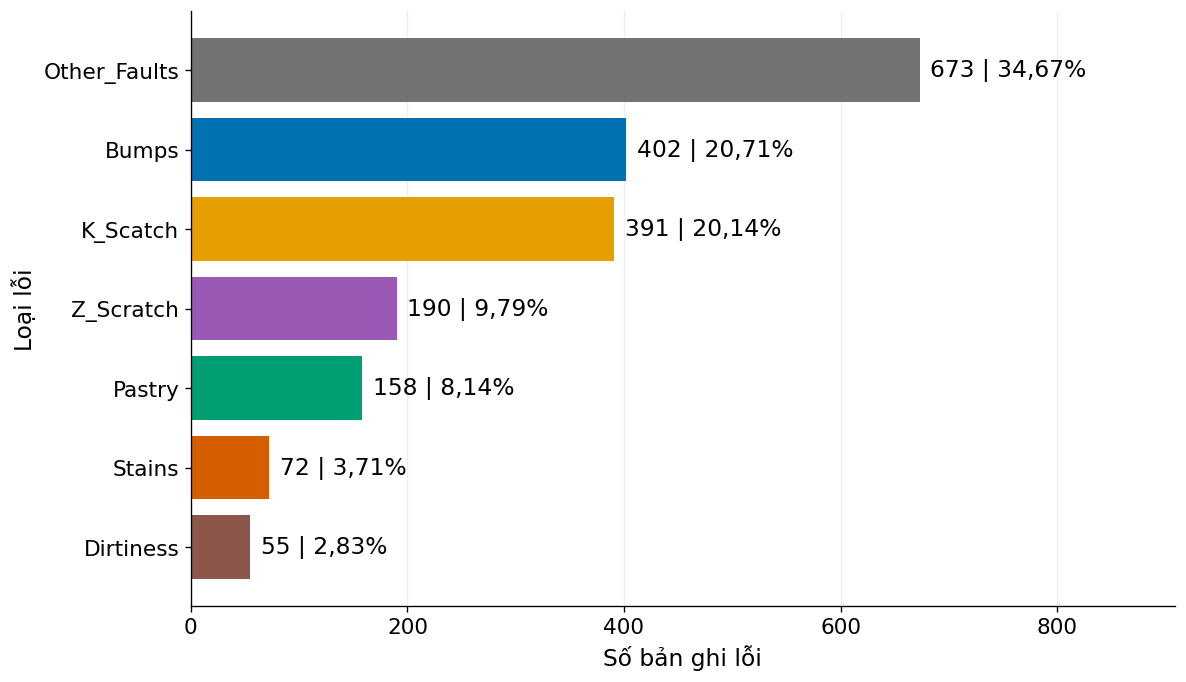
\includegraphics[width=\linewidth]{figures/chuong4/notebook_01_co_cau_loi.png}
\captionof{figure}{Other\_Faults đông nhất; Bumps và K\_Scatch chỉ chênh nhau 11 bản ghi}
\label{fig:ch4cocau}
\smallskip\par\footnotesize Nguồn: notebook bước 1--6, mục 5.2, Hình 1; 1.941 bản ghi sau làm sạch.
\end{minipage}\end{center}

\maCot{Other_Faults} đứng đầu với 673 bản ghi, chiếm 34,67\%. Tiếp theo là \maCot{Bumps} với 402 bản ghi (20,71\%) và \maCot{K_Scatch} với 391 bản ghi (20,14\%). Hai nhóm sau chỉ chênh nhau 11 bản ghi, tương đương khoảng 0,57 điểm phần trăm trên toàn tập. Ở cuối phân bố, \maCot{Dirtiness} có 55 bản ghi; cỡ mẫu lớn nhất gấp cỡ mẫu nhỏ nhất khoảng 12,24 lần.

Thứ hạng này cho thấy dữ liệu mất cân bằng giữa các nhãn. Nhóm đông sẽ tạo nhiều điểm hơn trên scatter, trong khi nhóm ít mẫu cần được đọc cùng cỡ mẫu khi so sánh phân bố. Riêng \maCot{Other_Faults} là nhãn gộp, chưa cho biết thành phần bên trong. Số lượng của nhóm vì vậy chưa xác định được một hiện tượng lỗi duy nhất để ưu tiên xử lý.

\begin{center}\begin{minipage}{\linewidth}
\centering
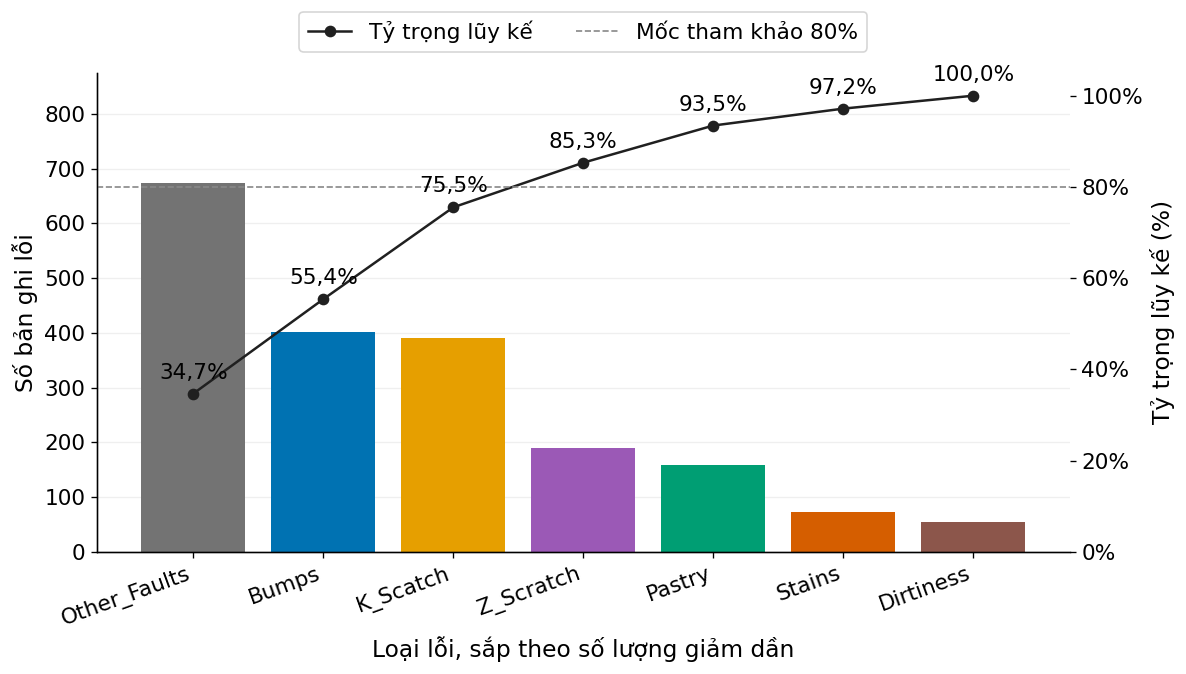
\includegraphics[width=\linewidth]{figures/chuong4/notebook_02_pareto_loi.png}
\captionof{figure}{Ba nhãn đầu chiếm 75,53\%; cần bốn nhãn để vượt mốc 80\%}
\label{fig:ch4pareto}
\smallskip\par\footnotesize Nguồn: notebook bước 1--6, mục 5.2, Hình 2; lũy kế theo số bản ghi lỗi.
\end{minipage}\end{center}

Đường lũy kế trong Hình~\ref{fig:ch4pareto} đặt mức tập trung đó vào toàn bộ cơ cấu. Ba nhãn đầu chứa 1.466 bản ghi, tương ứng 75,53\%; thêm \maCot{Z_Scratch} với 190 bản ghi thì lũy kế đạt 85,32\%. Mốc 80\% giúp đọc phạm vi bao phủ của các nhãn phổ biến, nhưng chưa có chi phí hay mức hạ cấp sản phẩm để chuyển thứ hạng này thành ưu tiên sản xuất. Để hiểu hai nhóm gần bằng nhau về tần suất, phần tiếp theo xét chúng nằm ở dòng thép nào.

\section{Q2: Bumps và K\_Scatch phân bố khác nhau theo dòng thép}
\label{sec:ch4q2}

Hình~\ref{fig:ch4thepsoluong} chia mỗi nhãn thành A300 và A400. Màu biểu diễn nhãn, họa tiết phân biệt dòng thép. Tổng cỡ mẫu là 777 bản ghi A300 và 1.164 bản ghi A400.

\begin{center}\begin{minipage}{\linewidth}
\centering
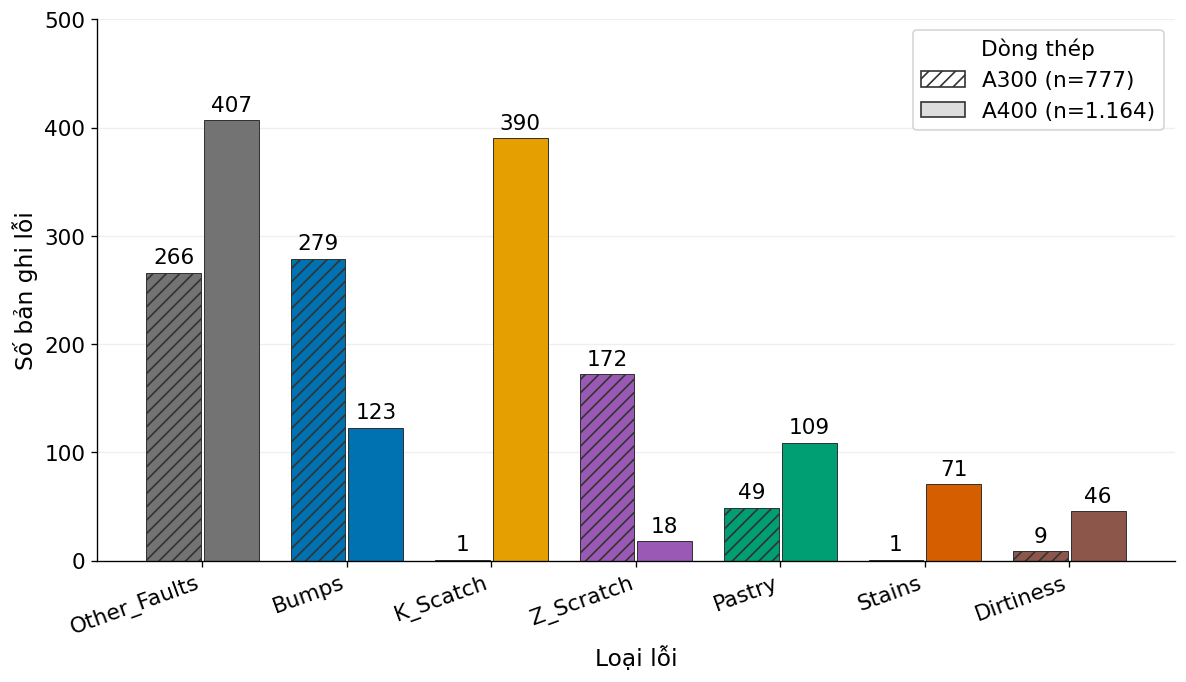
\includegraphics[width=\linewidth]{figures/chuong4/notebook_03_loi_theo_thep_so_luong.png}
\captionof{figure}{K\_Scatch gần như tập trung ở A400; Bumps có mặt đáng kể ở cả hai dòng thép}
\label{fig:ch4thepsoluong}
\smallskip\par\footnotesize Nguồn: notebook bước 1--6, mục 5.3, Hình 3; số đếm theo tổ hợp nhãn--dòng thép.
\end{minipage}\end{center}

\maCot{Bumps} gồm 279 bản ghi A300 và 123 bản ghi A400. Với \maCot{K_Scatch}, phân bố là một bản ghi A300 và 390 bản ghi A400. Dù số lượng toàn tập gần nhau, hai nhãn có vị trí rất khác trong bảng chéo. Ngoài \maCot{K_Scatch}, \maCot{Stains} tập trung ở A400 và \maCot{Z_Scratch} tập trung ở A300; cả ba vượt mốc mô tả 90\% trong từng nhãn theo công thức~\eqref{eq:tieuchiq2}.

\begin{center}\begin{minipage}{\linewidth}
\captionof{table}{Phân bố theo dòng thép cho thấy ba nhãn tập trung trên 90\%}
\label{tab:ch4taptrung}
\small\setstretch{1.1}
\begin{tabularx}{\linewidth}{@{}Y rrr r@{}}
\toprule
Nhãn & Tổng & A300 & A400 & \shortstack{Tỷ trọng ở dòng\\tập trung (\%)} \\
\midrule
\maCot{Other_Faults} & 673 & 266 & 407 & 60,48 (A400) \\
\maCot{Bumps} & 402 & 279 & 123 & 69,40 (A300) \\
\maCot{K_Scatch} & 391 & 1 & 390 & \textbf{99,74} (A400) \\
\maCot{Z_Scratch} & 190 & 172 & 18 & \textbf{90,53} (A300) \\
\maCot{Pastry} & 158 & 49 & 109 & 68,99 (A400) \\
\maCot{Stains} & 72 & 1 & 71 & \textbf{98,61} (A400) \\
\maCot{Dirtiness} & 55 & 9 & 46 & 83,64 (A400) \\
\bottomrule
\end{tabularx}
\smallskip\par\raggedright\footnotesize Mẫu số tỷ trọng là tổng bản ghi của từng nhãn; số liệu từ mục 5.3, bảng hỗ trợ Hình 3 trong notebook.
\end{minipage}\end{center}

Để so sánh cơ cấu khi hai dòng thép có cỡ mẫu khác nhau, Hình~\ref{fig:ch4theptytrong} đưa từng dòng về 100\%. Mẫu số lúc này chuyển sang tổng bản ghi lỗi của dòng thép đang xét.

\begin{center}\begin{minipage}{\linewidth}
\centering
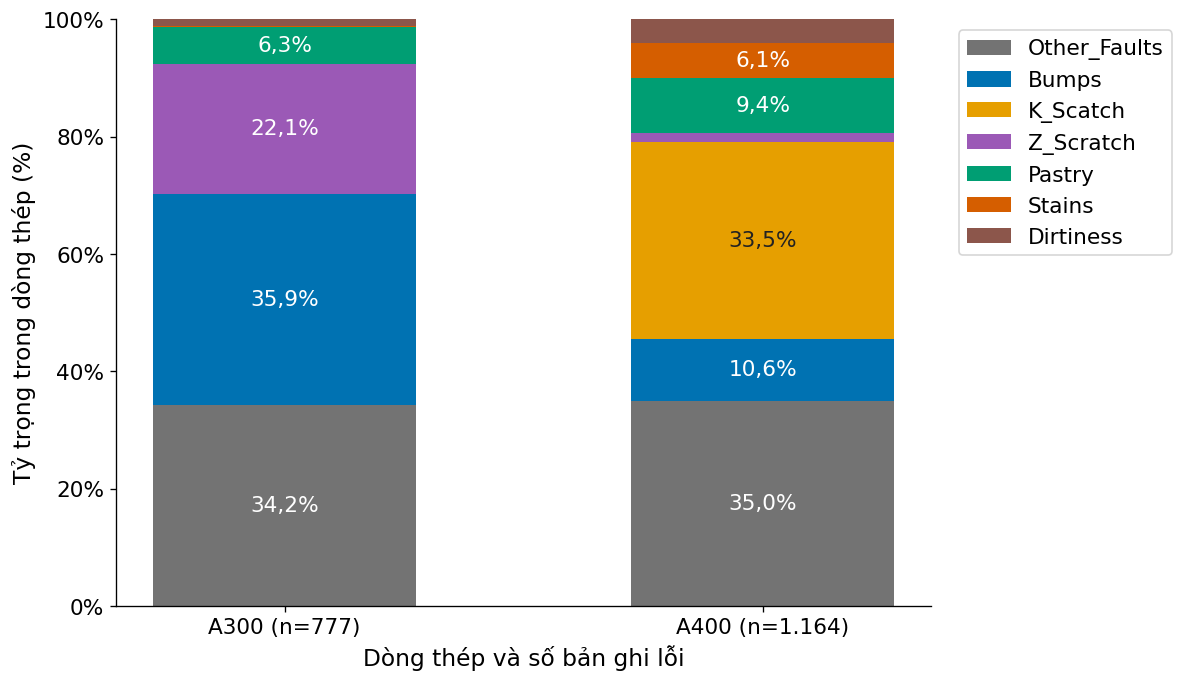
\includegraphics[width=\linewidth]{figures/chuong4/notebook_04_loi_theo_thep_ty_trong.png}
\captionof{figure}{Trong tập lỗi, A300 nổi bật Bumps và Z\_Scratch; A400 nổi bật K\_Scatch}
\label{fig:ch4theptytrong}
\smallskip\par\footnotesize Nguồn: notebook bước 1--6, mục 5.3, Hình 4; mỗi dòng thép cộng 100\%.
\end{minipage}\end{center}

Ở A300, \maCot{Bumps} chiếm 35,91\% và \maCot{Z_Scratch} chiếm 22,14\%. Ở A400, \maCot{K_Scatch} chiếm 33,51\%, còn \maCot{Bumps} chiếm 10,57\%. Tỷ trọng \maCot{Other_Faults} gần nhau, lần lượt 34,23\% và 34,97\%; khác biệt nổi bật nằm ở các nhãn cụ thể.

Với cùng 390 bản ghi \maCot{K_Scatch}/A400, phép chia $390/391$ cho 99,74\% mô tả dòng thép trong nhãn, còn $390/1.164$ cho 33,51\% mô tả nhãn trong dòng thép. Cả hai đều có mẫu số là bản ghi lỗi. Thiếu tổng sản lượng, chúng chưa cho biết xác suất phát sinh lỗi của A400. Sự tập trung quan sát được dẫn đến câu hỏi tiếp theo: đặc trưng độ sáng có giúp mô tả nhóm này cụ thể hơn không?

\section{Q3: Độ sáng tối thiểu làm rõ khác biệt ở phần trung tâm}
\label{sec:ch4q3}

Hình~\ref{fig:ch4scatter} đặt mỗi bản ghi tại cặp độ sáng tối thiểu--tối đa, giữ bảy màu nhãn và giảm độ đậm để thấy vùng chồng điểm. Các điểm \maCot{K_Scatch} màu cam tập trung nhiều về phía độ sáng tối thiểu thấp; nhiều nhãn khác cùng xuất hiện ở vùng trung tâm.

\begin{center}\begin{minipage}{\linewidth}
\centering
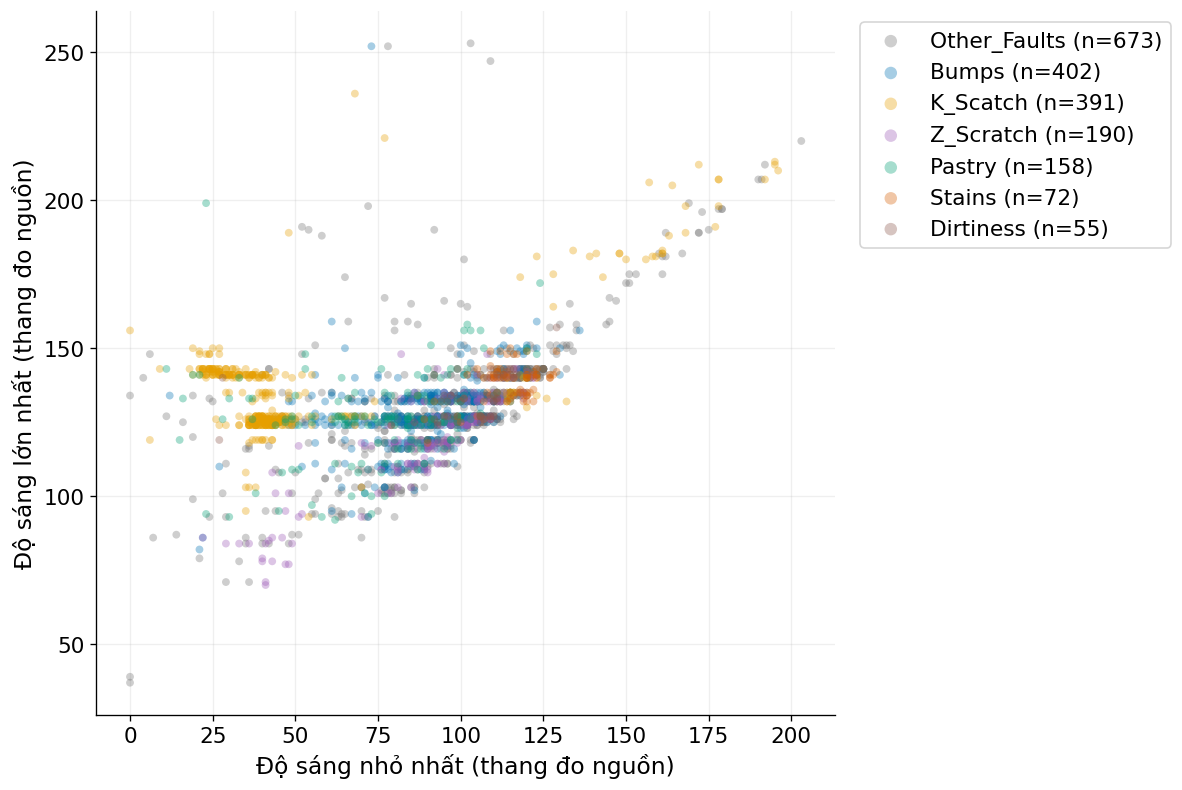
\includegraphics[width=\linewidth]{figures/chuong4/notebook_05_scatter_do_sang.png}
\captionof{figure}{K\_Scatch tập trung về phía độ sáng tối thiểu thấp, nhưng các điểm vẫn chồng lấn}
\label{fig:ch4scatter}
\smallskip\par\footnotesize Nguồn: notebook bước 1--6, mục 5.4, Hình 5; mỗi điểm là một bản ghi.
\end{minipage}\end{center}

Trung vị độ sáng tối thiểu của \maCot{K_Scatch} là 41, trong khi sáu nhãn còn lại có trung vị từ 80 đến 115. Khoảng P25--P75 của nhóm là 35--49; cận dưới nhỏ nhất của sáu khoảng còn lại là 64 ở \maCot{Pastry}. Bảng~\ref{tab:ch4dosang} giúp đọc chính xác phần trung tâm mà scatter khó thể hiện do điểm chồng nhau.

\begin{center}\begin{minipage}{\linewidth}
\captionof{table}{Phần trung tâm độ sáng tối thiểu của K\_Scatch khác biệt rõ hơn độ sáng tối đa}
\label{tab:ch4dosang}
\small\setstretch{1.1}
\begin{tabularx}{\linewidth}{@{}Y r p{2.3cm}r p{2.1cm}@{}}
\toprule
Nhãn & \shortstack{Trung vị\\Min} & P25--P75 Min & \shortstack{Trung vị\\Max} & P25--P75 Max \\
\midrule
\maCot{Other_Faults} & 97 & 80--111 & 127 & 119--140 \\
\maCot{Bumps} & 91 & 79,25--102 & 127 & 124--134 \\
\maCot{K_Scatch} & 41 & \textbf{35--49} & 134 & 126--141 \\
\maCot{Z_Scratch} & 93 & 81--104 & 124 & 111--132 \\
\maCot{Pastry} & 80 & 64--94 & 126 & 119--133 \\
\maCot{Stains} & 115 & 110--120 & 140 & 135--142 \\
\maCot{Dirtiness} & 107 & 96,5--111 & 132 & 127--140 \\
\bottomrule
\end{tabularx}
\smallskip\par\raggedright\footnotesize Min/Max: độ sáng tối thiểu/tối đa trên thang nguồn; thống kê từ mục 5.4, phần ``Tương quan và thống kê theo nhãn'' trong notebook.
\end{minipage}\end{center}

Khác biệt này chỉ áp dụng cho 50\% trung tâm. Toàn bộ độ sáng tối thiểu của \maCot{K_Scatch} trải từ 0 đến 196, vẫn chồng phạm vi của các nhóm khác; 297/391 bản ghi của nhãn có Min dưới 50 (75,96\%). Ở độ sáng tối đa, IQR 126--141 cũng chồng với nhiều nhãn. Vì vậy, dấu hiệu Min thấp là căn cứ lựa chọn đặc trưng để kiểm chứng, chưa tạo thành một ngưỡng gán nhãn.

Hệ số Pearson toàn tập là 0,4296, mô tả liên hệ tuyến tính dương giữa Min và Max. Giá trị này chưa đo khả năng phân loại lỗi. Tiêu chí không chồng IQR được bổ sung sau khi quan sát dữ liệu; cần đánh giá trên tập độc lập trước khi dùng cho nhận diện. Sau độ sáng, độ dày cung cấp thêm một chiều để xem sự tập trung của \maCot{K_Scatch} có đi cùng đặc điểm vật liệu hay không.

\section{Q4: Độ dày của K\_Scatch tập trung hẹp, thống kê gộp cần đọc cùng dòng thép}
\label{sec:ch4q4}

Hình~\ref{fig:ch4doday} là boxplot độ dày theo nhãn trên toàn tập, chưa tách A300/A400. \maCot{Other_Faults} có hộp rộng, trong khi hộp của \maCot{K_Scatch}, \maCot{Z_Scratch} và \maCot{Stains} co lại thành vạch vì P25 bằng P75.

\begin{center}\begin{minipage}{\linewidth}
\centering
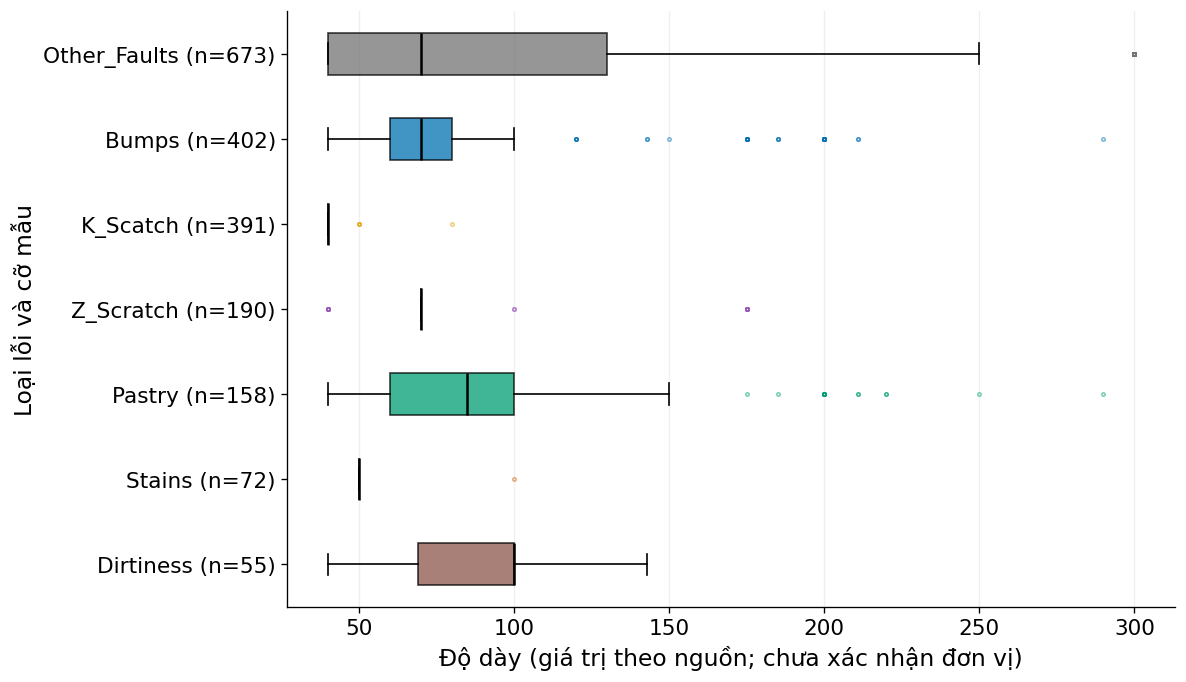
\includegraphics[width=\linewidth]{figures/chuong4/notebook_06_boxplot_do_day.png}
\captionof{figure}{K\_Scatch tập trung ở độ dày 40; Other\_Faults phân tán rộng hơn}
\label{fig:ch4doday}
\smallskip\par\footnotesize Nguồn: notebook bước 1--6, mục 5.5, Hình 6; độ dày theo thang nguồn, chưa xác nhận đơn vị.
\end{minipage}\end{center}

Toàn tập có trung vị độ dày 70 và 76,30\% bản ghi nằm trong khoảng 40--80. \maCot{K_Scatch} có trung vị 40, IQR bằng 0 và độ lệch chuẩn mẫu 2,20. Với \maCot{Other_Faults}, P25--P75 là 40--130; với \maCot{Bumps}, khoảng này là 60--80. IQR bằng 0 chưa đồng nghĩa với không biến thiên: \maCot{Z_Scratch} có IQR bằng 0 tại 70 nhưng độ lệch chuẩn mẫu vẫn là 24,70.

\begin{center}\begin{minipage}{\linewidth}
\captionof{table}{Trung vị gộp có thể che khác biệt độ dày giữa A300 và A400}
\label{tab:ch4doday}
\small\setstretch{1.1}
\setlength{\tabcolsep}{4pt}
\begin{tabularx}{\linewidth}{@{}Y r p{1.8cm}r p{2.2cm}p{2.2cm}@{}}
\toprule
Nhãn & \shortstack{Trung vị\\gộp} & P25--P75 & SD mẫu & \shortstack{A300\\Trung vị (N)} & \shortstack{A400\\Trung vị (N)} \\
\midrule
\maCot{Other_Faults} & 70 & 40--130 & 73,85 & 80 (266) & 50 (407) \\
\maCot{Bumps} & 70 & 60--80 & 38,05 & 70 (279) & 40 (123) \\
\maCot{K_Scatch} & 40 & 40--40 & 2,20 & 80 (1) & 40 (390) \\
\maCot{Z_Scratch} & 70 & 70--70 & 24,70 & 70 (172) & 175 (18) \\
\maCot{Pastry} & 85 & 60--100 & 51,59 & 80 (49) & 90 (109) \\
\maCot{Stains} & 50 & 50--50 & 5,89 & 100 (1) & 50 (71) \\
\maCot{Dirtiness} & 100 & 69--100 & 28,66 & 69 (9) & 100 (46) \\
\bottomrule
\end{tabularx}
\smallskip\par\raggedright\footnotesize Nguồn: mục 5.5 trong notebook, bảng hỗ trợ Hình 6 và ``Bảng bổ sung. Độ dày tách theo dòng thép''. N là cỡ mẫu; N=1 chỉ mô tả một bản ghi.
\end{minipage}\end{center}

Bảng bổ sung của notebook cho thấy \maCot{Bumps} có trung vị 70 ở A300 và 40 ở A400; \maCot{Other_Faults} có trung vị tương ứng 80 và 50. Đây là thông tin từ thống kê nhóm, bổ sung cho boxplot gộp. Hai tổ hợp \maCot{K_Scatch}/A300 và \maCot{Stains}/A300 chỉ có một quan sát; trung vị 175 của \maCot{Z_Scratch}/A400 cũng chỉ dựa trên 18 bản ghi.

Kết hợp Q2 và Q4 cho thấy dòng thép và độ dày đi cùng nhau rất chặt trong nhóm \maCot{K_Scatch}. Dữ liệu chưa đủ để tách ảnh hưởng riêng của từng yếu tố; thiếu sản lượng cũng chưa cho phép kết luận độ dày nào dễ phát sinh lỗi. Đặc điểm tiếp theo được xét là diện tích, nơi hai nhóm gần bằng nhau về số lượng có thể khác nhau nhiều về quy mô vùng lỗi.

\section{Q5: Diện tích làm rõ khác biệt và giải thích quyết định giữ các cờ IQR}
\label{sec:ch4q5}

Diện tích trải trên nhiều bậc độ lớn nên Hình~\ref{fig:ch4boxarea} dùng trục log cơ số 10. Boxplot vẫn được tính từ \maCot{Pixels_Areas} trên thang gốc, rồi mới đổi trục hiển thị. Khoảng cách bằng nhau trên trục thể hiện tỷ số bằng nhau; các điểm ngoài râu được giữ lại.

\begin{center}\begin{minipage}{\linewidth}
\centering
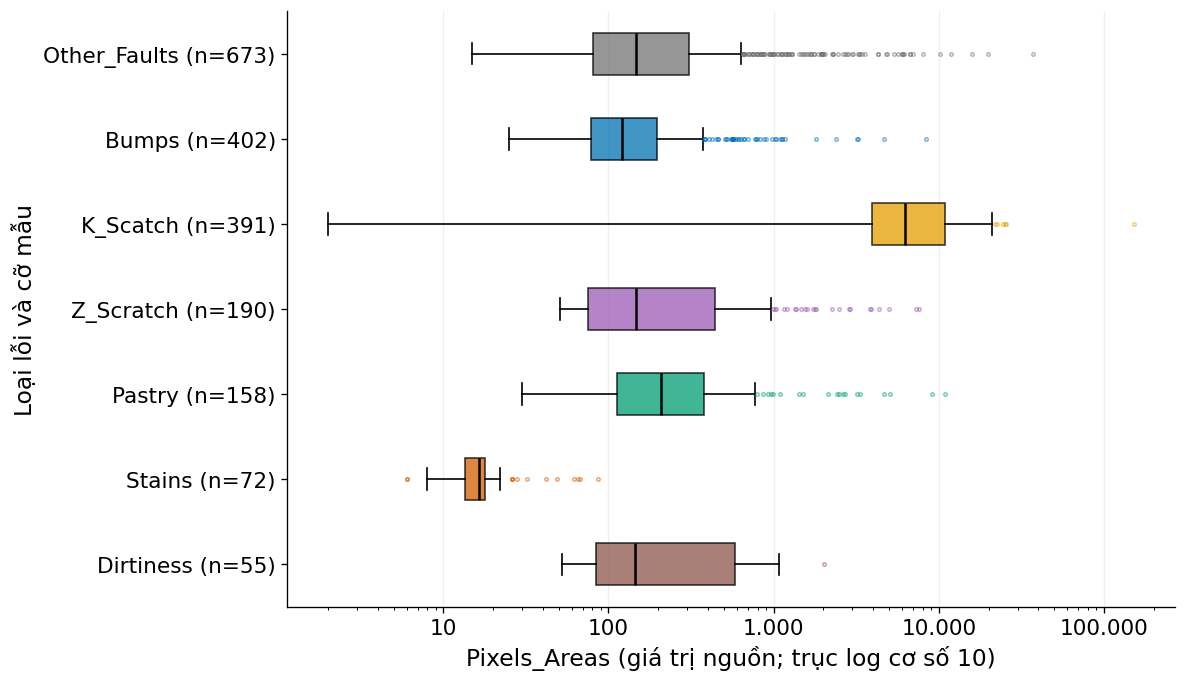
\includegraphics[width=\linewidth]{figures/chuong4/notebook_07_boxplot_dien_tich_log.png}
\captionof{figure}{K\_Scatch và Stains ở hai đầu của phân bố diện tích trung tâm}
\label{fig:ch4boxarea}
\smallskip\par\footnotesize Nguồn: notebook bước 1--6, mục 5.5, Hình 7; boxplot tính trên diện tích gốc, trục hiển thị log.
\end{minipage}\end{center}

Trung vị diện tích của \maCot{K_Scatch} là 6.281, lớn hơn khoảng 52,12 lần trung vị 120,5 của \maCot{Bumps}. \maCot{Stains} có trung vị nhỏ nhất, 16,5. IQR của \maCot{K_Scatch} là 3.948,5--10.908,5, nằm cao hơn IQR của các nhóm còn lại; \maCot{Stains} có IQR 13,5--18, nằm thấp hơn. Các nhãn ở giữa chồng nhau nhiều, nên diện tích đơn lẻ chưa mô tả đầy đủ khác biệt giữa chúng.

\begin{center}\begin{minipage}{\linewidth}
\captionof{table}{K\_Scatch có 326 cờ IQR toàn tập nhưng chỉ sáu điểm ngoài râu riêng của nhãn}
\label{tab:ch4area}
\small\setstretch{1.1}
\setlength{\tabcolsep}{4pt}
\begin{tabularx}{\linewidth}{@{}Y r p{3.0cm}rr@{}}
\toprule
Nhãn & Trung vị & P25--P75 & \shortstack{Ngoài râu\\từng nhãn} & \shortstack{Cờ IQR\\toàn tập} \\
\midrule
\maCot{Other_Faults} & 146 & 81--308 & 103 & 42 \\
\maCot{Bumps} & 120,5 & 78,25--197,5 & 44 & 5 \\
\maCot{K_Scatch} & 6.281 & 3.948,5--10.908,5 & \textbf{6} & \textbf{326} \\
\maCot{Z_Scratch} & 146 & 75,25--442 & 23 & 10 \\
\maCot{Pastry} & 209 & 112,5--381,25 & 19 & 11 \\
\maCot{Stains} & 16,5 & 13,5--18 & 13 & 0 \\
\maCot{Dirtiness} & 145 & 84,5--581,5 & 1 & 1 \\
\midrule
Tổng số bản ghi theo tiêu chí & & & 209 & 395 \\
\bottomrule
\end{tabularx}
\smallskip\par\raggedright\footnotesize Nguồn: mục 5.5, bảng hỗ trợ Hình 7 trong notebook. Điểm ngoài râu vượt hàng rào 1,5 × IQR tính riêng từng nhãn; cờ IQR toàn tập dùng một hàng rào chung cho 1.941 bản ghi.
\end{minipage}\end{center}

Phần trung tâm khác biệt chưa có nghĩa mọi quan sát đều tách nhau: diện tích \maCot{K_Scatch} trải từ 2 đến 152.655. Diện tích lớn cũng chưa đo được mức thiệt hại, vì dữ liệu thiếu tiêu chí chấp nhận và thông tin hạ cấp sản phẩm.

Hai cột cuối Bảng~\ref{tab:ch4area} trả lời vế giá trị ngoài râu của Q5: có 209 bản ghi nằm ngoài râu khi tính riêng từng nhãn, so với 395 cờ theo ngưỡng toàn tập. Riêng \maCot{K_Scatch}, 326/391 bản ghi bị gắn cờ toàn tập (83,38\%), nhưng chỉ 6/391 bản ghi nằm ngoài râu của chính nhãn (1,53\%). Chênh lệch này cho thấy nhiều bản ghi có diện tích lớn so với toàn tập vẫn nằm trong phạm vi râu của nhóm có diện tích trung tâm lớn.

Nếu loại tự động toàn bộ cờ, tập còn 1.546 dòng và \maCot{K_Scatch} còn 65 bản ghi, chỉ chiếm 4,20\%, thay vì 20,14\% ban đầu. Đây là phép đối chiếu giả định từ số cờ, không phải dữ liệu đã dùng để vẽ hình. Nó cho thấy ngưỡng chung có thể loại phần lớn một nhóm vốn có diện tích trung tâm lớn. Quyết định giữ các giá trị khớp nguồn ở Q0 vì vậy giúp bảo toàn đặc điểm đã quan sát.

\section{Đối chiếu kết quả trên dashboard và phạm vi kiểm thử}
\label{sec:ch4dashboard}

Dashboard cho phép chọn dòng thép, nhãn và khoảng độ dày rồi tính lại KPI, biểu đồ và bảng trên cùng tập con. Mục 6.3 ``Giao diện, bộ lọc và KPI'' của notebook kiểm tra bốn phạm vi ở Bảng~\ref{tab:ch4kpi}; mục 6.2, phần ``Đối chiếu cùng đầu vào với notebook bước 3--5'', đối chiếu bảng lỗi, cơ cấu, hai mẫu số tỷ trọng và thống kê đặc trưng với module dùng trong ứng dụng.

Hình~\ref{fig:ch4dashboard} ghi lại giao diện ứng dụng đang chạy khi chọn A400 và \maCot{K_Scatch}, giữ khoảng độ dày 40--300 của toàn nguồn. Bộ lọc và bốn KPI cùng xuất hiện trên màn hình, giúp đối chiếu phạm vi đang chọn với dòng tương ứng trong Bảng~\ref{tab:ch4kpi}.

\begin{center}\begin{minipage}{\linewidth}
\centering
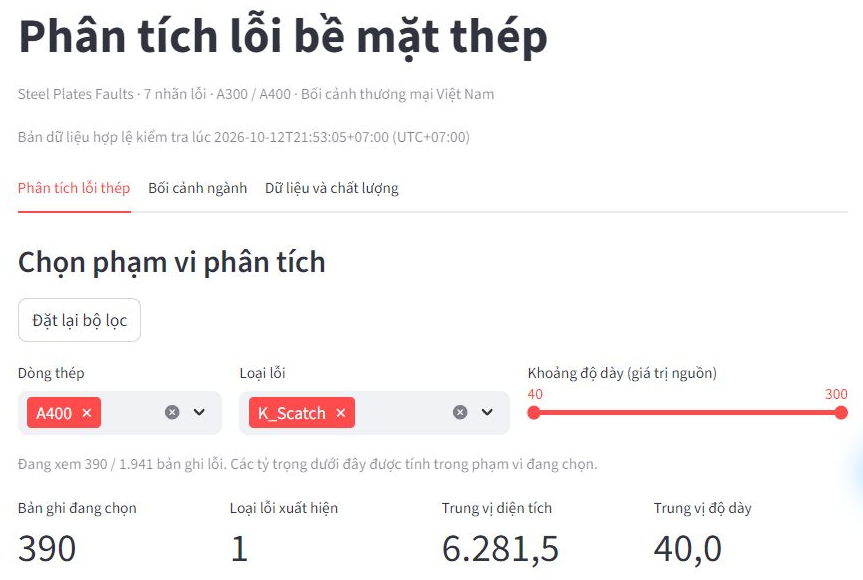
\includegraphics[width=\linewidth]{figures/chuong4/dashboard_a400_kscatch.png}
\captionof{figure}{Dashboard A400 và K\_Scatch: 390 bản ghi, một nhãn, trung vị diện tích 6.281,5 và độ dày 40,0}
\label{fig:ch4dashboard}
\smallskip\par\footnotesize Nguồn: ảnh chụp ứng dụng Streamlit đang chạy tại máy cục bộ ngày 12/10/2026; KPI được đối chiếu với mục 6.3 trong notebook.
\end{minipage}\end{center}

\begin{center}\begin{minipage}{\linewidth}
\captionof{table}{KPI theo phạm vi lọc nhất quán với các kết quả phân tích}
\label{tab:ch4kpi}
\small\setstretch{1.1}
\begin{tabularx}{\linewidth}{@{}Y rrrr@{}}
\toprule
Phạm vi & \shortstack{Số bản\\ghi} & \shortstack{Số\\nhãn} & \shortstack{Trung vị\\diện tích} & \shortstack{Trung vị\\độ dày} \\
\midrule
Toàn bộ & 1.941 & 7 & 174,0 & 70,0 \\
A300 & 777 & 7 & 113,0 & 70,0 \\
A400 và \maCot{K_Scatch} & 390 & 1 & 6.281,5 & 40,0 \\
Không chọn nhãn & 0 & 0 & -- & -- \\
\bottomrule
\end{tabularx}
\end{minipage}\end{center}

Khi thu hẹp vào A400 và \maCot{K_Scatch}, trung vị diện tích là 6.281,5 và trung vị độ dày là 40. Chênh lệch nhỏ với trung vị diện tích 6.281 ở Q5 đến từ việc bỏ bản ghi duy nhất của nhãn trên A300. Với tập rỗng, trung vị không xác định nên được để trống trong bảng tính và hiển thị dấu gạch trên giao diện.

Lần chạy lại bộ kiểm thử ngày 12/10/2026 lúc 21 giờ 53 phút (UTC+7) ghi nhận 11 ca đạt, không có lỗi, thất bại hay ca bỏ qua; kết quả được lưu tại \maCot{outputs/buoc_6/test_results.json} và đối chiếu trong mục 6.6 ``Kiểm tra ứng dụng'' của notebook. Các ca kiểm tra pipeline, bộ lọc, phạm vi rỗng, nạp nguồn và giữ bản hợp lệ, đồng thời xác nhận bốn KPI ở phạm vi A400 và \maCot{K_Scatch} khớp Bảng~\ref{tab:ch4kpi}. Lỗi API và chu kỳ cập nhật được mô phỏng; thử thay tệp thực hiện trên bản sao riêng. Kết quả này xác nhận hành vi trong các tình huống đã thử. Đánh giá với người dùng và theo dõi cập nhật dài hạn vẫn cần thực hiện thêm.

\section{Thảo luận và tiểu kết}
\label{sec:ch4thaoluan}

Qua bảy hình, \maCot{K_Scatch} chuyển từ nhãn phổ biến thứ ba thành một nhóm có các đặc điểm quan sát cụ thể: gần như tập trung ở A400, độ dày có trung vị 40 và phân tán hẹp, độ sáng tối thiểu thấp ở phần trung tâm, diện tích trung tâm lớn. \maCot{Bumps} có số lượng gần bằng nhưng trải trên cả hai dòng thép và diện tích nhỏ hơn nhiều. Những khác biệt này giúp chọn tổ hợp cần khảo sát; chúng chưa xếp hạng mức nghiêm trọng của lỗi.

\maCot{Stains} cũng có đặc điểm đáng chú ý: 71/72 bản ghi thuộc A400, trung vị độ dày 50 và trung vị diện tích 16,5. Với \maCot{Other_Faults}, số lượng lớn và phân bố rộng gợi ý cần làm rõ định nghĩa nhãn bằng ảnh bề mặt và thông tin QC trước khi phân chia nhóm. Các hướng này xuất phát từ mô tả trong mẫu, cần bằng chứng ngoài dữ liệu hiện tại để xác nhận.

Ba giới hạn chi phối cách sử dụng kết quả. Thứ nhất, thiếu tổng sản lượng và định danh tấm/cuộn khiến tỷ trọng bản ghi lỗi chưa trở thành tỷ lệ sản phẩm lỗi, đồng thời tính độc lập giữa các quan sát chưa được xác nhận. Thứ hai, thiếu biến vận hành và dữ liệu trong các tổ hợp dòng thép--độ dày nên chưa xác định nguyên nhân hoặc tách ảnh hưởng của từng yếu tố. Thứ ba, ngày là mô phỏng, đơn vị vật lý chưa được xác nhận đầy đủ và các tiêu chí khám phá được bổ sung sau khi xem dữ liệu.

Nguồn thương mại không có khóa liên hệ với các bản ghi lỗi, nên chỉ cung cấp bối cảnh độc lập, không giải thích những phân bố trong chương. Bước hoàn thiện tiếp theo là bổ sung sản lượng, định danh sản phẩm, thời gian thực, ảnh lỗi và mức thiệt hại; kiểm chứng dấu hiệu độ sáng trên tập độc lập; đồng thời đánh giá dashboard bằng nhiệm vụ sử dụng cụ thể. Việc giữ dữ liệu có căn cứ nguồn và ghi rõ mẫu số là cơ sở để các bước đó tiếp tục từ kết quả hiện tại.

Chương 4 đã nối kiểm tra dữ liệu với một câu chuyện phân tích từ cơ cấu nhãn đến đặc trưng từng nhóm. Hai nhãn \maCot{Bumps} và \maCot{K_Scatch} gần nhau về tần suất nhưng khác rõ ở dòng thép và diện tích trung tâm; độ sáng và độ dày bổ sung căn cứ mô tả. Đối chiếu 326 cờ toàn tập với sáu điểm ngoài râu riêng của \maCot{K_Scatch} làm rõ vì sao cần xem xét cấu trúc nhóm trước khi xử lý ngoại lai. Các kết quả xác lập những nội dung cần kiểm chứng tiếp và được chuyển thành phạm vi lọc có thể đối chiếu trên dashboard.
